\section{Shape Sensitivity Analysis for 1D problem}
% ================================================
For the first benchmark case, we looked at the flow between two plates that was defined in Section \ref{sec:C3_benchmark_case}. The governing equation and boundary conditions for this problem is shown in Equation \eqref{eq:C4_1DbenchmarkProblem}. The boundary condition is defined as $u = U$ at $y = L$.

\begin{subequations}\label{eq:C4_1DbenchmarkProblem}
\begin{equation}\label{eq:C4_1DbenchmarkGoverningEquation}
    u_t = \mu u_{yy} \quad \text{in } \Omega_f
\end{equation}
\begin{equation}\label{eq:C4_1DbenchmarkBoundaryCondition}
\begin{cases}
    u = U \quad \text{at } y = L \\
    u = 0 \quad \text{at } y = 0
\end{cases}
\end{equation}
\end{subequations}

The analytical result for the steady-state velocity profile between the two plates is defined in Equation \eqref{eq:C4_1DbenchmarkAnalyticalSolution}

\begin{equation}\label{eq:C4_1DbenchmarkAnalyticalSolution}
	u = \frac{Ux}{L}
\end{equation}

This enables us to treat the moving wall velocity ($U$) and the distance between the two plates ($L$) as design variables. The sensitivity of steady-state velocity profile between the two plate to these design variables are calculated using CSA. The results of the CSA are verified with the analytical sensitivity results in Equation \eqref{eq:C4_1DbenchmarkAnalyticalSensitivityResults}.

\begin{subequations}\label{eq:C4_1DbenchmarkAnalyticalSensitivityResults}
\begin{equation}\label{eq:C4_1DbenchmarkAnalyticalSAlength}
	\frac{\partial u}{\partial L} = -\frac{Ux}{L^2}
\end{equation}
\begin{equation}\label{eq:C4_1DbenchmarkAnalyticalSAvelocity}
	\frac{\partial u}{\partial U} = \frac{x}{L}
\end{equation}
\end{subequations}

For this benchmark problem, the flow is modeled using two different immersed boundary techniques introduced in the beginning of this chapter, penalization method and the virtual boundary method. This difference between the analysis of flow from Chapter \ref{ch:immersedBoundary} is the use of RH and RD functions instead of discontinuous step and delta function. Therefore, first the effect of these modifications are investigated on the simulation results.

For the flow simulation using the penalization method of Equation \eqref{eq:C4_NSwithPenalization} we investigated effect of node number and the moving wall velocity of the accuracy of the solution. To have a stable solution, the time step of flow analysis cannot be bigger that $2 / \kappa$ where $\kappa$ is the porosity value that is selected to model the solid domain. For this analysis the $\eta$ value of the RH function is selected based on the criteria that 99 percent change of the RH function occurs within one mesh cell. The result for the simulation based on RH function is compared with the step function in Figure \ref{fig:C4_effectOfRHfunctionOnSimulationResults1Dproblem}.

\begin{figure}[H]
	\centering
	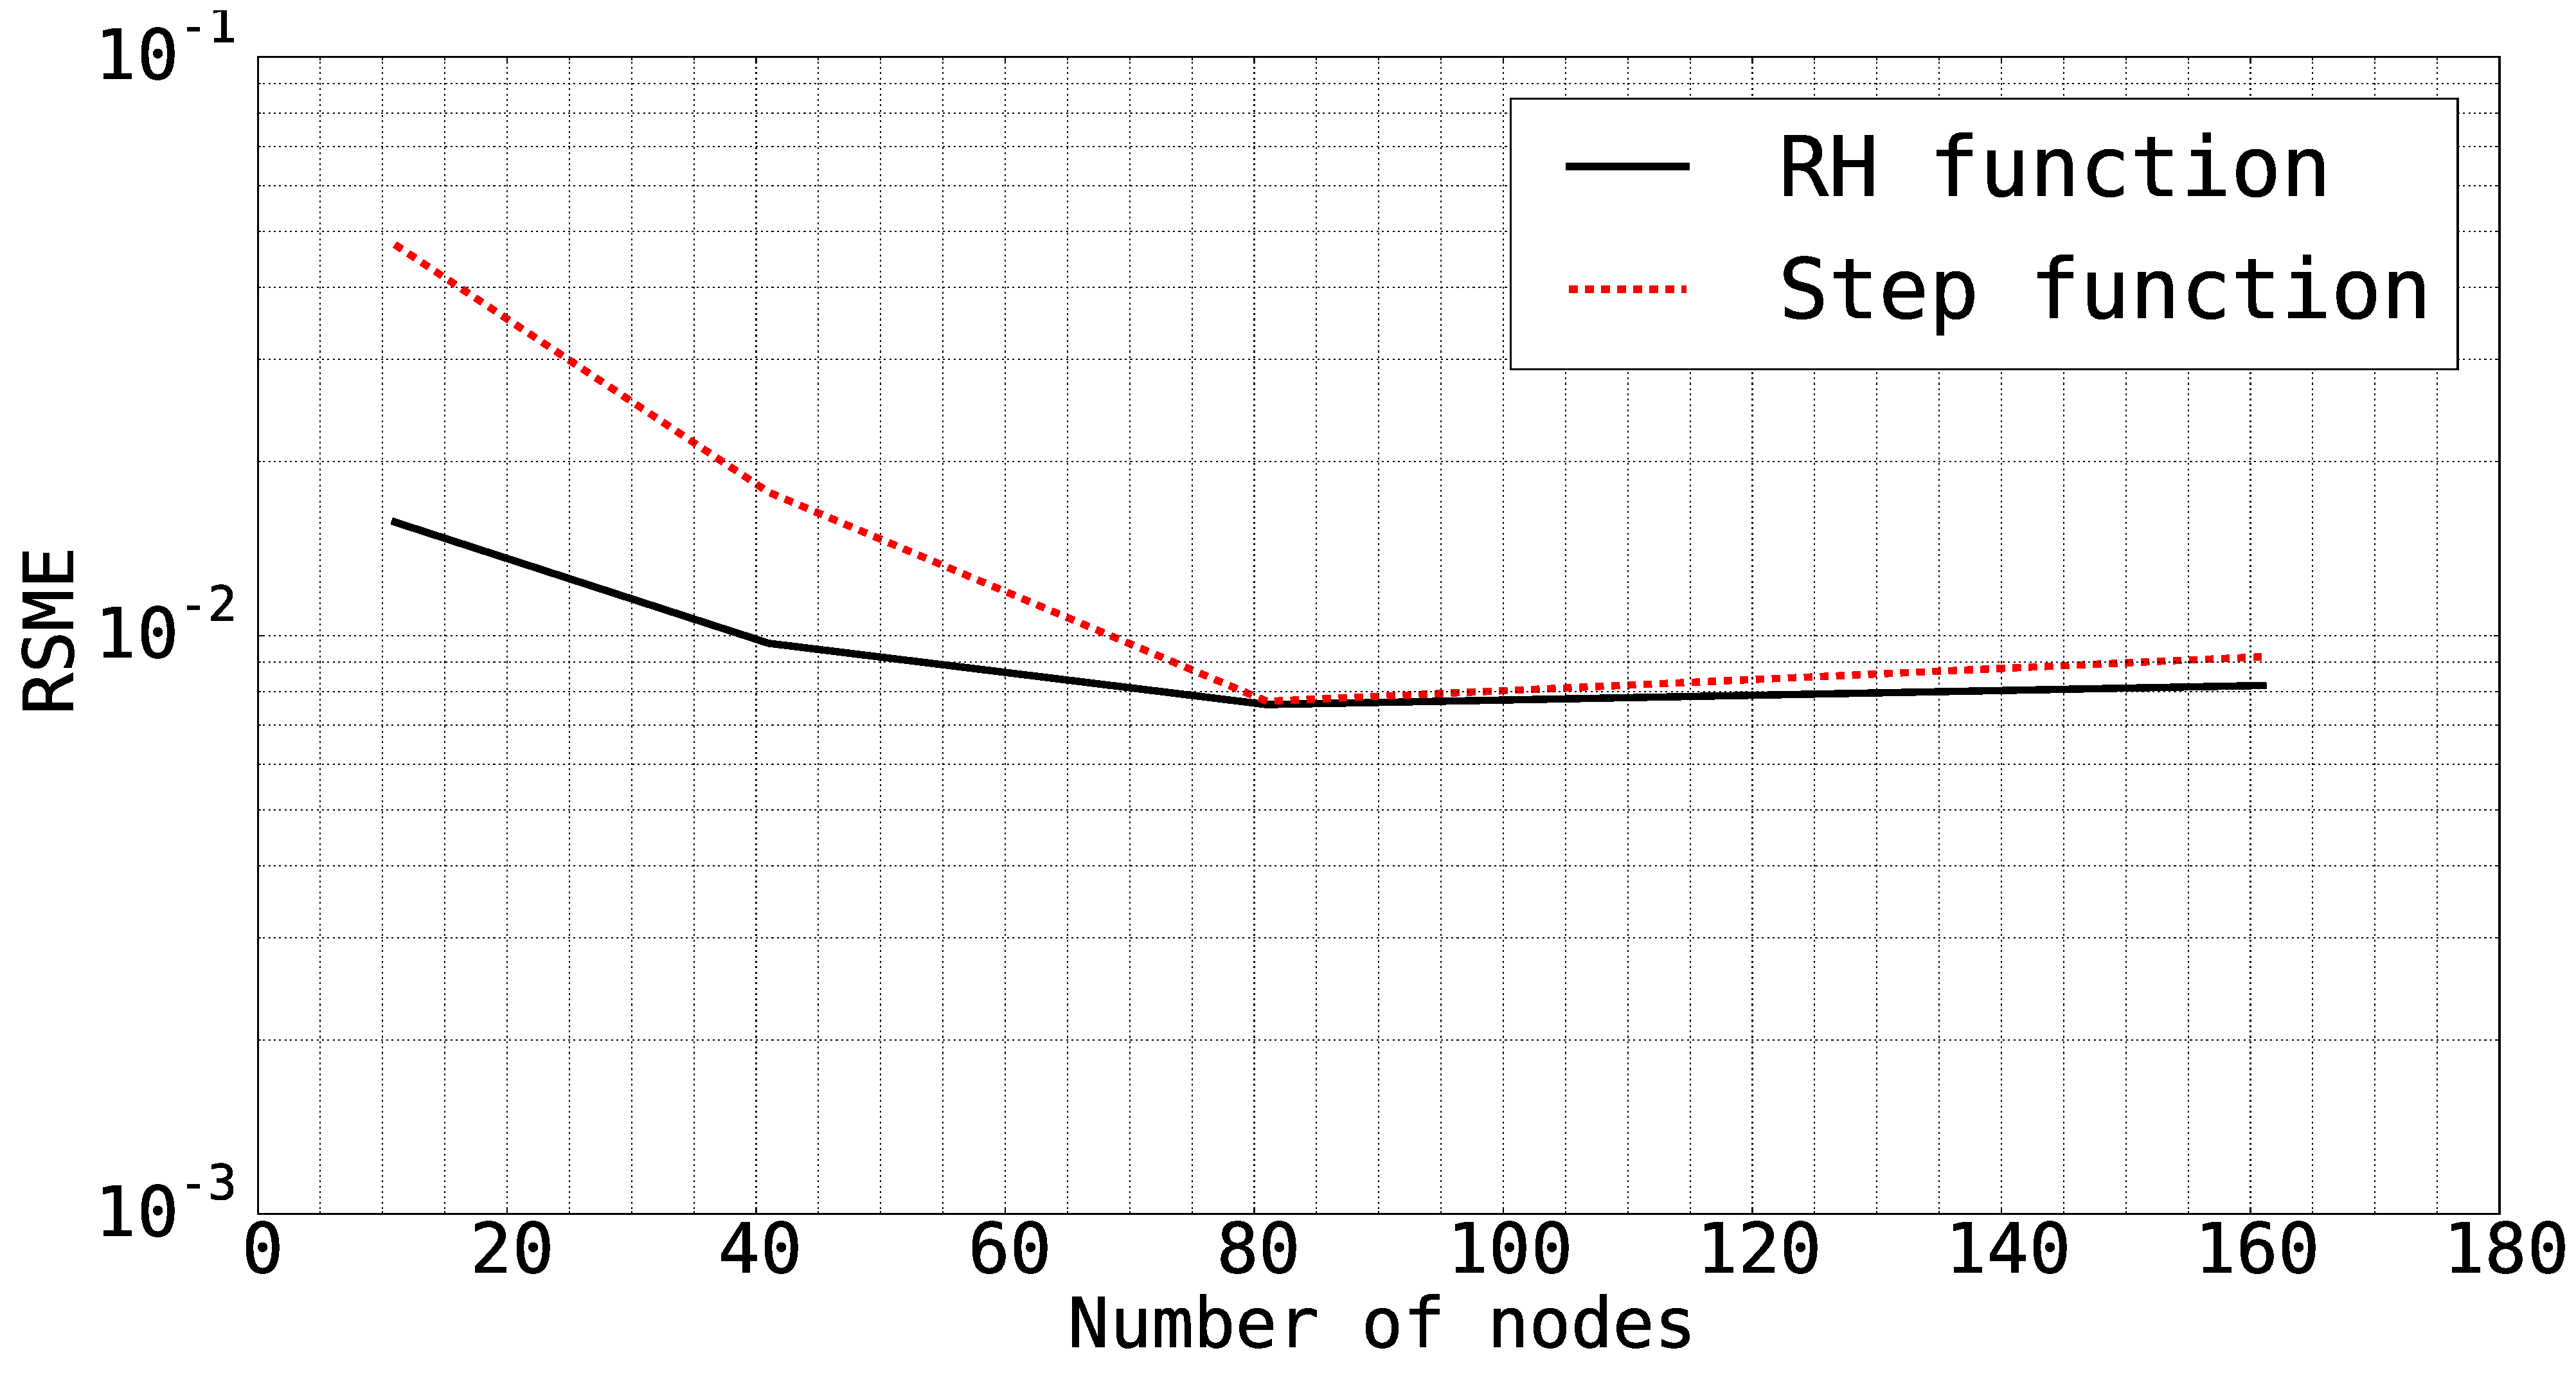
\includegraphics[width=12.00cm]{Chapter_4/figure/effect_of_RH_on_simulation_vs_numberOfNodes_1D_problem.eps}
	\caption{Effect of Regularized Heaviside (RH) and step function on the solution accuracy.}
	\label{fig:C4_effectOfRHfunctionOnSimulationResults1Dproblem}
\end{figure}

As shown in Figure \ref{fig:C4_effectOfRHfunctionOnSimulationResults1Dproblem}, the result of the RH function are more accurate compared to the step function. The effect of wall velocity of the accuracy of the simulation was also investigated. The wall velocity was selected as $1 m/s$, $10 m/s$, $100 m/s$, and $1000 m/s$. However, this did not affect the accuracy of the simulation.

The sensitivity equations for the penalization technique are derived by differentiating the governing equation as shown in Equation \eqref{eq:C4_NSwithPenalizationIBsensitivity}. However, for this problem the convective terms and pressure gradient drop out resulting in the sensitivity equation as shown in Equation \eqref{eq:C4_SAforPenlizationMethod1D}.

\begin{equation}\label{eq:C4_SAforPenlizationMethod1D}
	\frac{\partial u'}{\partial t} = 
	\mu \frac{\partial^2 u'}{\partial x^2} +
	\kappa \left[
	\frac{\partial \mathcal{H}}{\partial X} \frac{\partial X}{\partial b} + 
	\mathcal{H}(X) u'
	\right]
\end{equation}

where $X$ is $x - x_w$ and $x_w$ is the location of the solid wall. $u$ is the flow velocity, $\mu$ is the viscosity, $\kappa$ is the porosity, and $\mathcal{H}$ is the RH function. $b$ corresponds to the generic design variable and $u'$ is the sensitivity of the flow field to the design variable $b$. The boundary conditions are derived by differentiating the Equation \eqref{eq:C4_1DbenchmarkBoundaryCondition} in total form. This is shown in Equation \eqref{eq:C4_SAboundaryConditionforPenlizationMethod1D}.

\begin{equation}\label{eq:C4_SAboundaryConditionforPenlizationMethod1D}
\begin{cases}
	u' = 0 \qquad \text{at } x = 0 \\
	u' = \dfrac{\partial u}{\partial x} \quad \text{at } x = L
\end{cases}
\end{equation}